\documentclass[serif,mathserif]{beamer}
\usepackage{amsmath, amsfonts, epsfig, xspace}
\usepackage{algorithm,algorithmic}
\usepackage{pstricks,pst-node}
\usepackage{moreverb}
\usepackage[normal,tight,center]{subfigure}
\setlength{\subfigcapskip}{-.5em}
\usepackage{beamerthemesplit}
\usetheme{lankton-keynote}

\author{S\'ebastien Bourdeauducq}

\title{Migen}
\subtitle{A Python toolbox for building complex digital hardware}

\date{2013}

\begin{document}

\maketitle

\begin{frame}
\begin{centering}

\includegraphics[width=5cm]{migen_logo.png} \\

\includegraphics[width=\textwidth]{migenblock.png}
\end{centering}
\end{frame}

\begin{frame}[fragile]
\frametitle{FHDL}
\begin{itemize}
\item Python as a meta-language for HDL
\begin{itemize}
\item Think of a \verb!generate! statement on steroids
\end{itemize}
\item Restricted to locally synchronous circuits (multiple clock domains are supported)
\item Designs are split into:
\begin{itemize}
\item synchronous statements $\Longleftrightarrow$ \verb!always @(posedge clk)! \\
(VHDL: \verb!process(clk) begin if rising_edge(clk) then!)
\item combinatorial statements $\Longleftrightarrow$ \verb!always @(*)! \\
(VHDL: \verb!process(all inputs) begin!)
\end{itemize}
\item Statements expressed using nested Python objects
\begin{itemize}
\item Various syntax tricks to make them look nicer \\
\textit{("internal domain-specific language")}
\end{itemize}
\end{itemize}
\end{frame}

\begin{frame}[fragile]
\frametitle{FHDL crash course}
\begin{itemize}
\item Basic element is \verb!Signal!.
\begin{itemize}
\item Similar to Verilog \verb!wire/reg! and VHDL \verb!signal!.
\end{itemize}
\item Signals can be combined to form expressions.
\begin{itemize}
\item e.g. \verb!(a & b) | c!
\end{itemize}
\item Signals have a \verb!eq! method that returns an assignment to that signal.
\begin{itemize}
\item e.g. \verb!x.eq((a & b) | c)!
\end{itemize}
\item User gives an execution trigger (combinatorial or synchronous to some clock) to assignments, and makes them part of a \verb!Module!.
\begin{itemize}
\item Control structures (\verb!If!, \verb!Case!) also supported.
\end{itemize}
\item Modules can be converted for synthesis or simulated.
\end{itemize}
\end{frame}

\begin{frame}[fragile]
\frametitle{Conversion for synthesis}
\begin{itemize}
\item FHDL is entirely convertible to synthesizable Verilog
\end{itemize}
\begin{verbatimtab}
>>> from migen.fhdl.std import *
>>> from migen.fhdl import verilog
>>> counter = Signal(16)
>>> o = Signal()
>>> m = Module()
>>> m.comb += o.eq(counter == 0)
>>> m.sync += counter.eq(counter + 1)
>>> print(verilog.convert(m, ios={o}))
\end{verbatimtab}
\end{frame}

\begin{frame}[fragile]
\begin{verbatimtab}
module top(input sys_rst, input sys_clk, output o);

reg [15:0] counter;

assign o = (counter == 1'd0);

always @(posedge sys_clk) begin
        if (sys_rst) begin
                counter <= 1'd0;
        end else begin
                counter <= (counter + 1'd1);
        end
end

endmodule
\end{verbatimtab}
\end{frame}

\begin{frame}[fragile]
\frametitle{Name mangling}
\begin{verbatimtab}
class Foo:
    def __init__(self):
        self.la = [Signal() for x in range(2)]
        self.lb = [Signal() for x in range(3)]
a = [Foo() for x in range(3)]

-> foo0_la0, foo0_la1, foo0_lb0, foo0_lb1, foo1_la0, ...,
  foo1_lb0, ..., foo2_lb2
\end{verbatimtab}
\end{frame}

\begin{frame}
\centering 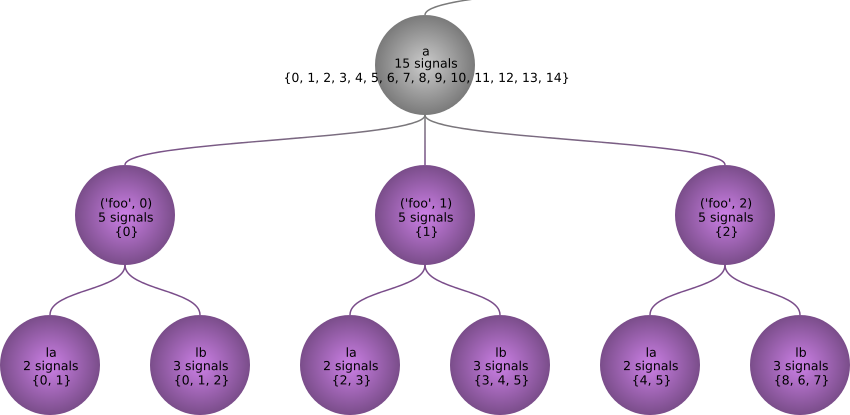
\includegraphics[width=\textwidth]{name_mangling.png}
\end{frame}

\begin{frame}[fragile]
\frametitle{Simulation}
\begin{itemize}
\item Modules can have a Python functions to execute at each clock cycle during simulations.
\item Simulator provide read and write methods that manipulate FHDL \verb!Signal! objects.
\item Powerful Python features, e.g. generators:
\end{itemize}
\begin{verbatimtab}
def my_generator():
        for x in range(10):
                t = TWrite(x, 2*x)
                yield t
                print("Wrote in " + str(t.latency) + " cycle(s)")
                # Insert some dead cycles to simulate bus inactivity.
                for delay in range(prng.randrange(0, 3)):
                        yield None
master1 = wishbone.Initiator(my_generator())
master2 = lasmibus.Initiator(my_generator(), port)
\end{verbatimtab}
\end{frame}

\begin{frame}[fragile]
\frametitle{Pytholite}
\begin{itemize}
\item Some of those generators are even synthesizable :)
\item Output: FSM + datapath
\item Lot of room for improvement (mapping, scheduling, recognized subset)
\item One application today: high-speed control of the analog RF chain of a radar
\end{itemize}
\begin{verbatimtab}
def generator():
        for i in range(10):
                yield TWrite(i, 0)
bus_if = wishbone.Interface()
pl = make_pytholite(generator,
        buses={"def": bus_if})
... verilog.convert(pl) ...
\end{verbatimtab}
\end{frame}

\begin{frame}[fragile]
\frametitle{Bus support}
\begin{itemize}
\item Wishbone\footnote{http://www.opencores.org}
\item SRAM-like CSR
\item DFI \footnote{http://www.ddr-phy.org}
\item LASMI
\end{itemize}
\centering 
\includegraphics[height=1cm]{opencores.png} 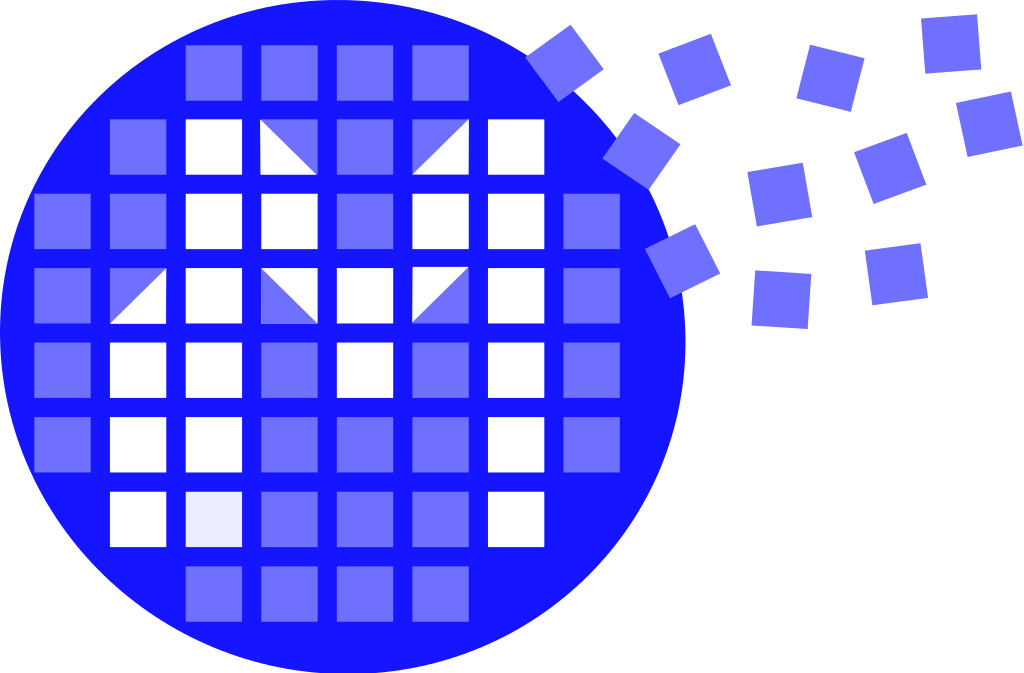
\includegraphics[height=1cm]{milkymist.png} 
\includegraphics[height=1cm]{dfi.png}
\begin{verbatimtab}
wishbonecon0 = wishbone.InterconnectShared(
        [cpu0.ibus, cpu0.dbus],
        [(lambda a: a[26:29] == 0, norflash0.bus),
         (lambda a: a[26:29] == 1, sram0.bus),
         (lambda a: a[26:29] == 3, minimac0.membus),
         (lambda a: a[27:29] == 2, wishbone2lasmi0.wishbone),
         (lambda a: a[27:29] == 3, wishbone2csr0.wishbone)])
\end{verbatimtab}
\end{frame}

\begin{frame}[fragile]
\frametitle{CSR banks and interrupt controllers}
\begin{verbatimtab}
_rxtx = CSR("rxtx", 8)
_divisor = CSRStorage("divisor", 16, reset=int(clk_freq/baud/16))
events = EventManager(_tx_event, _rx_event)
events.tx = EventSourceProcess()
events.rx = EventSourcePulse()
bank = csrgen.Bank([_rxtx, _divisor] + events.get_csrs(),
     address=address)
\end{verbatimtab}
\end{frame}

\begin{frame}
\frametitle{LASMI}
LASMI (Lightweight Advanced System Memory Infrastructure) key ideas
\begin{itemize}
\item Speed is beautiful: optimize for performance
\item Operate several FSMs (\textit{bank machines}) concurrently to manage each bank
\item Crossbar interconnect between masters and bank machines
\item Pipelining: new requests can be issued without waiting for data. Peak IO bandwidth (minus refresh) is attainable.
\item In a frequency-ratio system, issue multiple DRAM commands from different bank FSMs in a single cycle
\end{itemize}
\end{frame}

\begin{frame}
\frametitle{LASMIcon (milkymist-ng)}
Memory controller operates several \textit{bank machines} in parallel
\begin{itemize}
\item Each bank machine uses the page mode algorithm
\item Tracks open row, detects page hits
\item Ensures per-bank timing specifications are met (tRP, tRCD, tWR)
\item Generates DRAM-level requests (PRECHARGE, ACTIVATE, READ, WRITE)
\end{itemize}
\end{frame}

\begin{frame}
\frametitle{LASMIcon (milkymist-ng)}
\textit{Command steering} stage picks final requests
\begin{itemize}
\item In a frequency-ratio system, may issue multiple commands from several bank machines in a single cycle
\begin{itemize}
\item PHY uses SERDES to handle I/O
\item FPGAs are horribly and painfully SLOW, so we need such tricks even for DDR333 (2002!!!)
\end{itemize}
\item Groups writes and reads to reduce turnaround times (reordering)
\begin{itemize}
\item commands stay executed in-order for each bank machine: no reorder buffer needed on the master side
\end{itemize}
\item Ensures no read-to-write conflict occurs on the shared bidirectional data bus
\item Ensures write-to-read (tWTR) specification is met
\end{itemize}
\end{frame}

\begin{frame}
\frametitle{Migen support}
\begin{itemize}
\item Migen provides generic components only
\item e.g. memory controller and PHY are not included
\begin{itemize}
\item part of milkymist-ng\footnote{https://github.com/milkymist/milkymist-ng}
\item supports (hardware tested) SDR, DDR, LPDDR, DDR2 and DDR3 (partial) on Spartan-6
\end{itemize}
\item Provides containers, bus simulation components, crossbar interconnect
\end{itemize}
\end{frame}

\begin{frame}
\frametitle{Dataflow programming}
\begin{itemize}
\item Representation of algorithms as a graph (network) of functional units
\item Similar to Simulink or LabVIEW
\item Parallelizable and relatively intuitive
\item Migen provides infrastructure for actors (functional units) written in FHDL
\item Migen provides an actor library for DMA (Wishbone and LASMI), simulation, etc.
\end{itemize}
\end{frame}

\begin{frame}
Migen is open source!
\begin{itemize}
\item BSD
\begin{itemize}
\item Can be used in proprietary designs.
\item Contributing what you can is encouraged.
\end{itemize}
\item http://milkymist.org/3/migen.html
\item http://github.com/milkymist/migen
\item mailing list: http://lists.milkymist.org
\item IRC: Freenode \#milkymist
\end{itemize}

\centering 
\includegraphics[width=5cm]{migen_logo.png}

\end{frame}

\end{document}
